%\{ {\it  sp1d\_ch3\_2.tex} \}

\subsection {High order Polynomial Solution and Its Convergence}

In this section we construct a polynomial $P_n$ of order $n$ defined on $[0,1]$, which satisfies the following.
\begin{eqnarray}
\label{pois_scrv}
    P_n(0) = 0, &P_n(1) = 1 \\
    \frac{d^k}{dx^k}P_n(0) = 0, &\frac{d^k}{dx^k}P_n(1) = 0
\end{eqnarray}
for all $k = 1, \cdots, n-2$. \\
Then for each $n$, we obtain a polynomial $P_n$ by solving a system of linear equations having unique solution which determines the set of coefficients of $P_n$. We will apply the spectral polynomial solver to approximate the second derivative $Q_{n-2}$ of $P_n$.
The numerical and exact solutions by the solver we developed is shown in figure (\ref{scrvsol}).


\begin{figure}[h]
    \begin{center}
    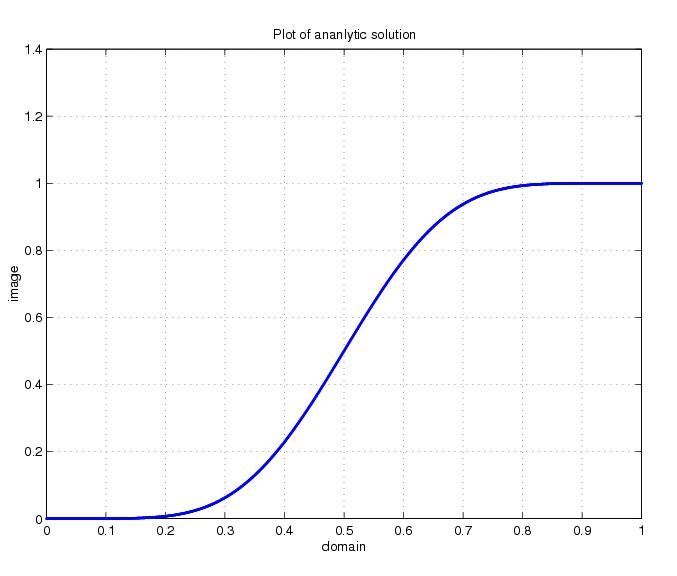
\epsfig{file = figs_dn/ScrvO_13.eps, width = 5cm}
    \caption{\label{scrvsol}Example of curve that satisfies conditions (\ref{pois_scrv}) with polynomial order $n=13$}
    \end{center}
\end{figure}
We will investigate the convergences by the h-type, p-type extension of trial functions below.

\begin{problem}
Consider the following differential equation for $u(x)$ such that
\begin{equation}
\label{poi_poly}
    \frac{d^2}{dx^2} u(x) = Q_{n-2},
\end{equation}
for all $x$ in $[0, 1]$ with the boundary condition defined in equation (\ref{pois_scrv}). Then the problem is to find approximation $u^{\delta}(x)$ of $u(x)$ using spectral polynomial method.
\end{problem}

Note that the accuracy of this interpolation satisfying equations (\ref{pois_scrv}) is dependent on the stability of matrix that defines the coefficients of interpolants. We used the Legendre basis function which is known to be more stable than monomials. In spite of this, there exists interpolation error close to $e^{-13}$. This cause the same amount of convergence error in p-type extension mode shown in right of Figure (\ref{ScrvconvDN}) and Table (\ref{hconv2t}).

\begin{itemize}

\item {Convergence h-type extension for equation (\ref{poi_poly})}

As we've seen in the case of equation (\ref{pois_sin}), in Figure (\ref{ScrvconvDN}), we see the error with respect to $L^{\infty}$ of the discrete solution to the equation is exponentially convergent to the size of element. This verifies the Log-Log scale of relation of theory (\ref{hrelation}).

\item {Convergence p-type extension for equation (\ref{poi_poly})}

This semi-Log scale plot also showing the exponential convergence of p-type extension of trial functions. Note that we approximate the finite order of polynomial. So there exists the lowest order $P_l$ that approximating with trial functions of order $P$ which $P > P_l$ should shows the same convergence as the case using trial functions of order $P_l$. In right of Figure (\ref{ScrvconvDN}), we can see the convergence is staying on approximation error which theoretically should be machine precision.

\end{itemize}

\begin{figure}[h]
\begin{center}
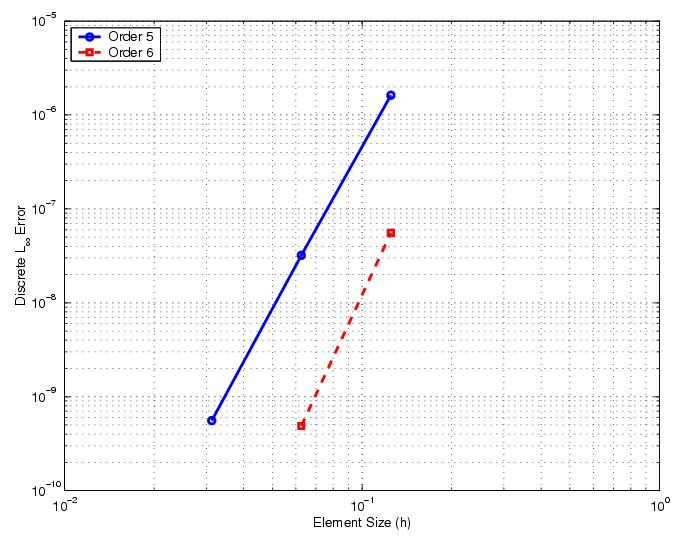
\epsfig{file = figs_dn/ScrvHconv.eps, width = 8.3cm}
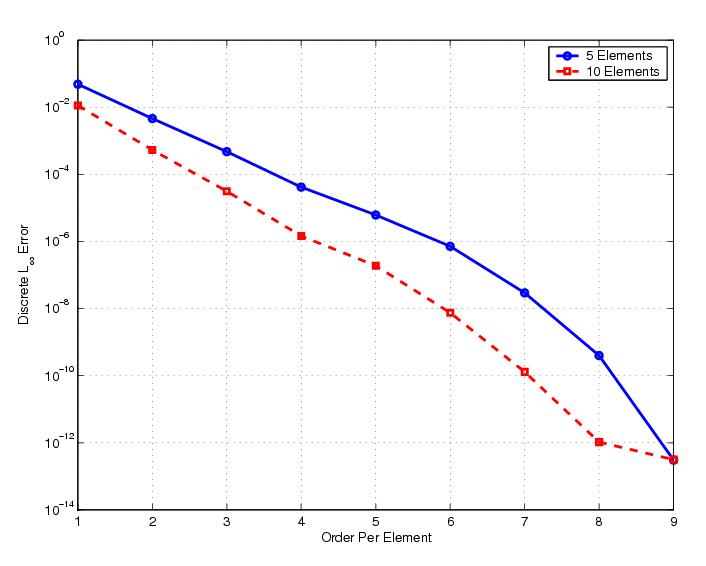
\epsfig{file = figs_dn/ScrvPconv.eps, width = 8.3cm}
\caption{\label{ScrvconvDN}
(Left)Convergence with respect to discrete $L^{\infty}$ norm as a function of size of elements. This test is performed using the h-type extension with fixed polynomial order 3, 4, and 5 respectively. Error on the Log-Log axis is demonstrating the algebraic convergence of the h-type extension.
(Right)Convergence w.r.t. $L^{\infty}$ norm as a function of size of polynomial order in semi-Log plot. It shows the exponential convergence of p-type extension for smooth solution. Two tests are performed for p-type extension with element length $0.2$ and $0.1$.
}
\end{center}
\end{figure}

\begin{table}[h]
\centering \caption{\label{hconv2t} This table shows the convergence of h-type resolution control done above Figure (\ref{ScrvconvDN}). We can see the slopes of each order $P$ is $P+1$ }
\begin{tabular}{|c|c|c|} \hline
    Polynomial order&Error($L^{\infty}$)&Slope   \\ \hline \hline
    3&$7.5530e-011$ &$3.9908$ \\ \hline
    4&$4.5619e-013$ &$4.6486$ \\ \hline
    5&$4.1855e-013$ &$5.7218$ \\ \hline
\end{tabular}
\hspace{.5in}
\begin{tabular}{|c|c|} \hline
    &\multicolumn{1}{|c|}{Error}\\
    \raisebox{0.5\baselineskip}%
    {Element Size}&($L^{\infty}$) \\ \hline \hline
    0.2&$3.0431e-013$  \\ \hline
    0.1&$3.1186e-013$ \\ \hline
\end{tabular}
\end{table}
